\subsection{Plotting}

\begin{frame}[fragile]
\begin{block}{}
\begin{minted}{python}
In [62]: plot([1,2,3])
In [63]: show()
\end{minted}
\end{block}
\begin{center}
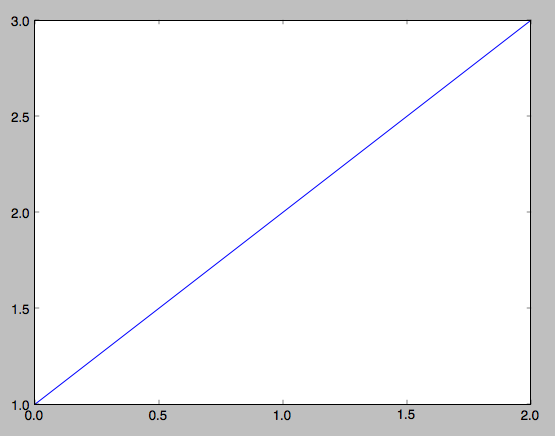
\includegraphics[scale=.35]{../figures/matplotlib/plot_basic.png}
\end{center}
\end{frame}

\begin{frame}[fragile]
\begin{block}{}
\begin{minted}{python}
In [69]: hold(False)

In [70]: plot([1,2,3], [.2, .3, .4], 'g+')

In [71]: plot([1,2,3], [.2, .3, .4], 'g+',
...           [2, 4, 6], [.2, .3, .4], 'bt')

In [72]: plot([1,2,3], [1,2,3], 'go-', label='line 1',
...           linewidth=2)
In [74]: hold(True)
In [75]: plot([1,2,3], [1,4,9], 'rs',  label='line 2')
In [76]: axis([0, 4, 0, 10])
In [77]: legend()
In [78]: save_fig(``my_file.png'')
\end{minted}
\end{block}
\end{frame}

